\chapter{Datos obtenidos}

Los audios recolectados tuvieron algunos problemas al grabarse. El principal problema fue que el ambiente que utilizó cada hablante no estaba completamente en silencio como para hacer una buena grabación. Muchos errores surgieron en esa dirección. Otros errores comunes pero no tan frecuentes fueron: interpretaciones erróneas de la consigna, errores de volumen del micrófono, saturación etc.. 

\subsection{Mediciones}

Escuchamos los audios para determinar si se realizaron correctamente. Los fuimos clasificando en: Conservar, Sonido saturado, Mucho ruido de fondo, Problema en el habla. Esta clasificación fue empírica, o sea no realizando ningún análisis sino que escuchando manualmente cada una. La cantidad de cada clase fue la siguiente:

\begin{table}[h]
\centering
\begin{tabular}{|l|c|c|c|c|}
\hline
\textbf{}  & \textbf{Bs.As. } & \textbf{Cba.} & \textbf{Total} \\ \hline
\textbf{Conservar}  & 222 & 105 & 327 \\ \hline
\textbf{Problemas en el habla}  & 33 & 15 & 48 \\ \hline
\textbf{Mucho ruido de fondo}  & 2 & 12 & 14 \\ \hline
\textbf{Sonido saturado}  & 2 & 0 & 2 \\ \hline
\end{tabular}
\end{table}

Algo importante de ver es que los datos obtenidos están desbalanceados. No pudimos obtener la misma cantidad de audios para los dos grupos. Esto se va a reflejar en la clasificación y en el análisis posterior.

\subsection{Errores comunes}

Las categorías establecidas anteriormente describen los errores comunes mas frecuentes. Podemos observar que del total de 391 grabaciones, 64 tuvo algún problema. Este es alrededor del 16\% de los audios grabados. Es un número alto para ser un experimento guiado. 

La gran causa de este número es la faltante de un chequeo en el mismo momento que va grabando cada uno de los audios. Un trabajo futuro sería analizar el audio grabado y rechazarlo si no supera un nivel aceptable auditivo. Esto puede implementarse de varias formas. Una posible sería cuando esta grabando medir el volumen del micrófono cada una cierta cantidad de tiempo, por ejemplo 1 segundo. Si en esa medición el volumen no se encuentra entre rango máximo y mínimo de volumen, descartar el audio y pedirle al hablante que vuelva a grabar.

%todo: esto nose si va mejor en Trabajos Futuros
También se le podría dar mas información al hablante. Sabiendo que el micrófono tuvo un pico de volumen se podría pedirle al hablante que no hable tan fuerte. Ídem si habla muy bajo. Otras posibles soluciones a este problema es analizar antes de empezar el experimento si el sonido ambiente es muy alto o no. Y luego de ello aceptar una grabación nueva. Todas esas soluciones e pueden realizar en la aplicación web sin intervenir en el servidor.

Para análisis mas precisos se puede aplicar mejores filtros cuando llega la grabación del lado del servidor. Cuando llega el mensaje del audio al servidor, este ya puede obtener el wav y realizarle todo tipo de análisis mas precisos. Recordemos que el servidor esta implementado en Python que posee muchas librerías útiles para el análisis de audios. Al momento de terminar el análisis del audio en cuestión, deberá enviar la respuesta al hablante informándole si se debe realizar devuelta la grabación o si fue exitosa. Es importante notar que esta solución necesita buena conexión para el server. 

Vamos a continuar con el análisis basándonos en los audios clasificados como Conservados. Luego trataremos de realizar algún análisis para reutilizar algunos de estos que tuvieron algún problema. 

\section{Alineación forzada}

El alineador automático no realiza su función de forma perfecta. Sucede que muchas veces alinea mal. Es muy importante descartar los audios mal alineados ya que sino cuando los procese el extractor nos darían información errónea. Fuimos chequeando cada audio y analizando si la alineación fue correcta con la aplicación Praat \cite{praat}. Para realizar esta tarea utilizamos el programa Praat. Los errores mas comunes fueron:
%todo citar bien a praat

\begin{itemize}
    \item \textbf{Ruido de fondo:} los casos donde el alineador se comporta de peor manera son los que se escuchan ruido de fondo. En esos casos las alineaciones resultan muy malas. Lamentablemente en nuestro caso esto es muy común. 

\begin{figure}[h!]
    \centerline{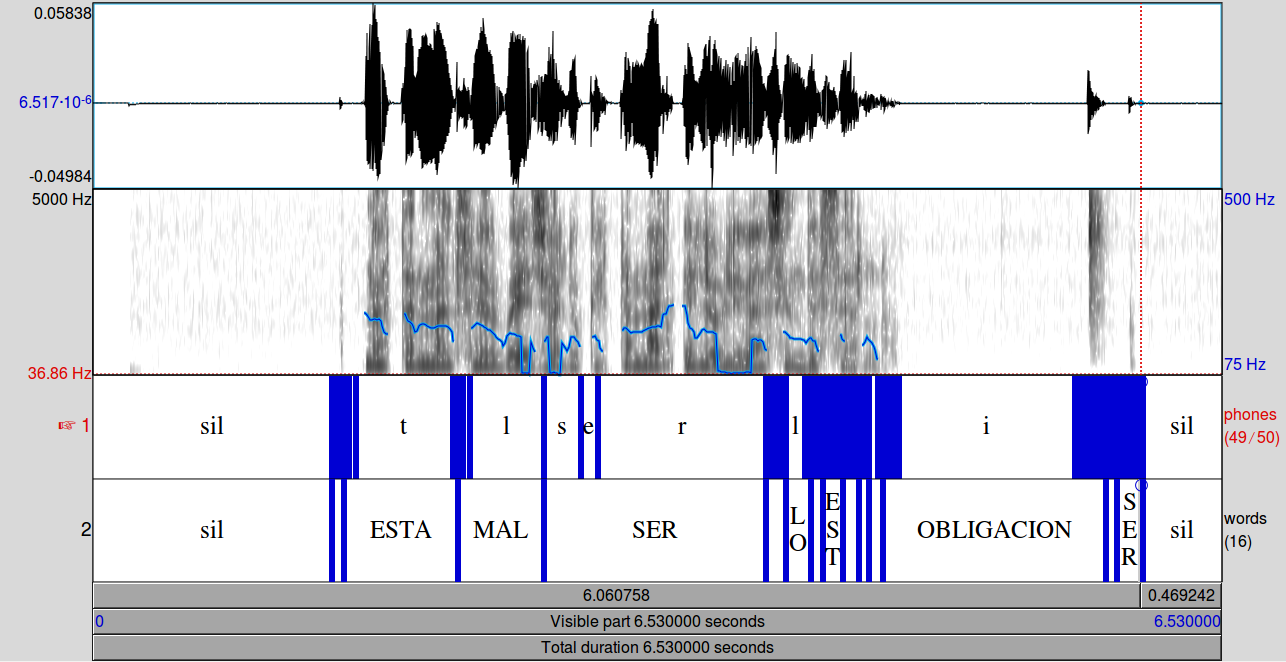
\includegraphics[width=0.8\textwidth]{alineacion_mala_inf} }
    \caption{Ejemplo de alineación mala por ruido}
\end{figure}

    \item \textbf{Mouse click al finalizar:} sucede que el ambiente donde los hablantes realizaban las grabaciones no estaba bien aislado. Pasó en muchas oportunidades que el click de finalizar del mouse se grabó como parte final de la grabación (Ver Fig. \ref{click_final}). Ese sonido se grabó y afectó la alineación de forma tal que se tomaba como habla.
    
\begin{figure}[h!]
    \centerline{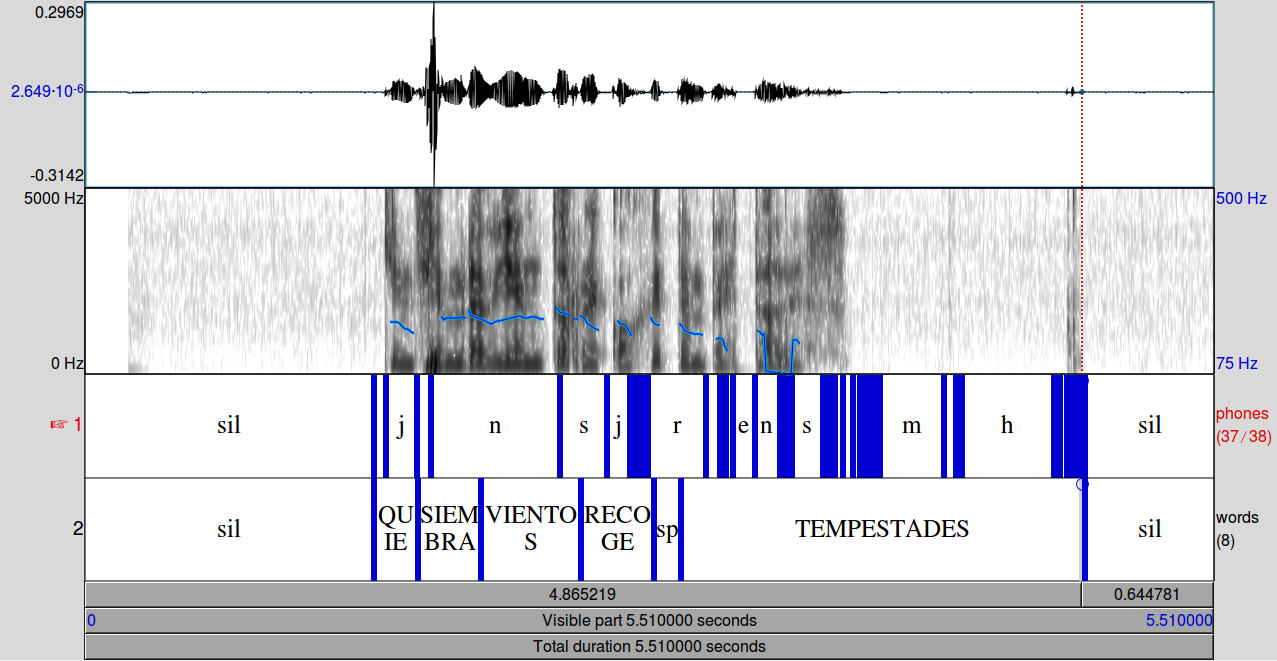
\includegraphics[width=0.8\textwidth]{click_al_final_inf} }
    \caption{Click al final}
    \label{click_final}
\end{figure}

    \item \textbf{Saturación del micrófono:} el volumen del micrófono es configurado por el hablante. Es por ello que debemos confiar en su buena voluntad. Sucede que muchas veces la grabación fue buena pero al final tuvo una entonación mas mucho mas fuerte que las demás, haciendo que posteriormente la alineación no sea precisa.

    \item \textbf{Estiramiento de la /s/ final:} en varias oportunidades se quiso exagerar la entonación. Las frases finalizadas en /s/ fueron grabadas en muchos casos sosteniendo ese fonema por tiempo prolongado. A pesar de que fue alineado correctamente en toda su duración, este fue llevado a una duración entendible. El problema que surgió en estos casos fue que el hablante no supo pronunciar la frase de la forma mas natural posible. Este fue el motivo por el cual se modificó.
\end{itemize}

\section{Corrección de errores}

Para corregir los errores descriptos debimos chequear cada uno de los textgrids. Los resultados de la cantidad de textgrid corregidos son:

\begin{table}[h]
\centering
\begin{tabular}{|l|c|c|c|c|}
\hline
\textbf{}  & \textbf{Bs.As. } & \textbf{Cba.} & \textbf{Total} \\ \hline
\textbf{Modificados}  & 101 & 88 & 189 \\ \hline
\textbf{Correctos sin modificación}  & 119 & 2 & 121 \\ \hline
\textbf{Total} & 220 & 90 & 310 \\ \hline
\end{tabular}
\end{table}

%todo: leer bien el mail de prosodylab
Esta forma se realizó ya que eran pocos audios pero en un experimento con más hablantes se debe utilizar la opción de '.SCORES' antes descripta. De estos 310 debemos sacar las grabaciones que se realizaron varias veces. Recordemos que cada hablante tenía la posibilidad de grabar varias veces la misma grabación con la idea de que la última va a ser la mejor. Debemos quitar estos casos para no contabilizar más de una vez la misma grabación. Los audios repetidos son alrededor de 50. Quitando estos podemos empezar con el análisis. 
